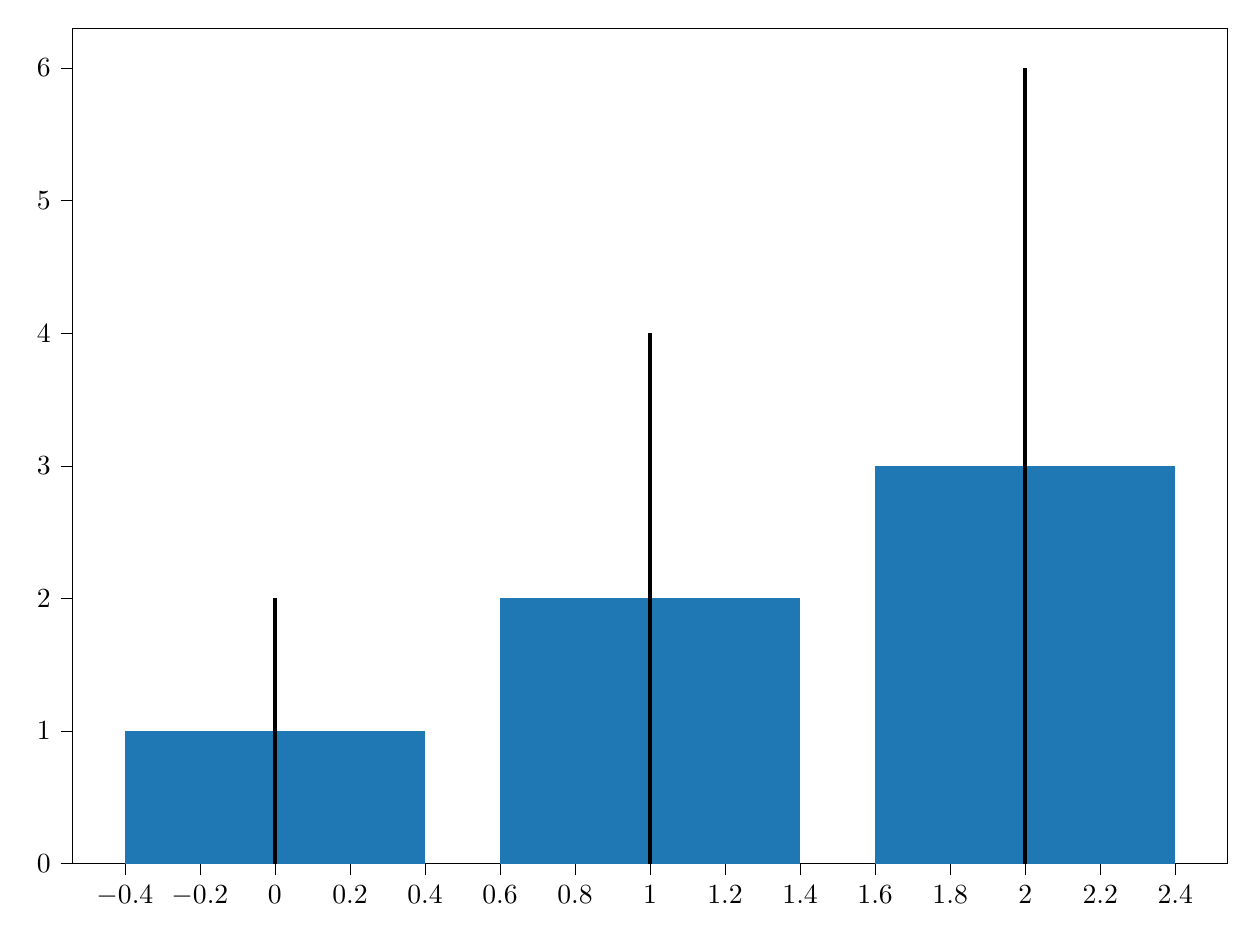
\begin{tikzpicture}

\definecolor{darkgray176}{RGB}{176,176,176}
\definecolor{steelblue31119180}{RGB}{31,119,180}

\begin{axis}[
height=4.8in,
tick align=outside,
tick pos=left,
width=6.4in,
x grid style={darkgray176},
xmin=-0.54, xmax=2.54,
xtick style={color=black},
y grid style={darkgray176},
ymin=0, ymax=6.3,
ytick style={color=black}
]
\draw[draw=none,fill=steelblue31119180] (axis cs:-0.4,0) rectangle (axis cs:0.4,1);
\draw[draw=none,fill=steelblue31119180] (axis cs:0.6,0) rectangle (axis cs:1.4,2);
\draw[draw=none,fill=steelblue31119180] (axis cs:1.6,0) rectangle (axis cs:2.4,3);
\path [draw=black, line width=1.5pt]
(axis cs:0,0)
--(axis cs:0,2);

\path [draw=black, line width=1.5pt]
(axis cs:1,0)
--(axis cs:1,4);

\path [draw=black, line width=1.5pt]
(axis cs:2,0)
--(axis cs:2,6);

\end{axis}

\end{tikzpicture}
